\documentclass[journal, twocolumn, transmag]{IEEEtran}

\usepackage[noindent]{ctex}
\renewcommand{\baselinestretch}{1.0}
\setmainfont[Ligatures=NoCommon]{TeX Gyre Termes}

\usepackage{amsmath,amsfonts}
\usepackage{graphicx}
\usepackage{booktabs}
\usepackage{cite}
\usepackage{xurl}
\usepackage[colorlinks,urlcolor=blue,linkcolor=blue,citecolor=blue]{hyperref}
\usepackage{lettrine}
\usepackage{fancyhdr}

\pagestyle{fancy}
\fancyhf{}
\chead{《深度学习和算法设计》课程大作业}
\cfoot{\thepage}
\renewcommand{\headrulewidth}{0pt}

\newcommand{\method}{VK-RCD}
\newcommand{\mmfi}{MM-Fi}
\newcommand{\xfi}{X-Fi}
\newcommand{\better}[1]{\textbf{#1}}
\newcommand{\smalltab}{\scriptsize}
\renewcommand{\refname}{REFERENCES}
\setlength{\tabcolsep}{3pt}
\renewcommand{\arraystretch}{1.05}

\begin{document}
\setlength{\parindent}{1em}

% ---------------- Title and author ----------------
\title{Privacy-Preserving Robust Multimodal Human Sensing with Visual-Keypoint Distillation}
\author{Liu Yige, 32561071, Dalian University of Technology\\
	\vspace{0.5cm}
}

% ---------------- Abstract and keywords ----------------
\IEEEtitleabstractindextext{
	\begin{abstract}
		Multimodal human sensing benefits from complementary RGB, depth, LiDAR, mmWave, and WiFi-CSI signals, but raw RGB introduces privacy risks and fixed-modality fusion is brittle when sensors are unavailable. This paper presents \method{}, a privacy-oriented and missing-modality robust framework built on the \mmfi{} human sensing setting. Instead of using raw RGB images, \method{} uses visual keypoints (VK) as a structured visual representation and combines them with non-visual sensing modalities. A full-modality teacher provides privileged supervision, while Student-VK is trained with random modality dropping to support arbitrary modality subsets. A non-visual Student-NV is further trained to evaluate deployment without any visual input. Reliability-aware fusion assigns adaptive decision weights to available modalities, reducing the influence of unreliable sensors. Experiments on human pose estimation (HPE) and human action recognition (HAR) show that Student-VK reduces HPE full-modality MPJPE from the official \xfi{} value of 83.70 mm to 50.17 mm and improves HAR full-modality accuracy from 72.20\% to 96.56\%. Cross-scene and cross-subject evaluations further show that the model is not limited to a single random split. The results demonstrate that privacy-preserving multimodal sensing can remain accurate under missing modalities, non-visual deployment, and environment shift.
	\end{abstract}

	\begin{IEEEkeywords}
		Deep learning, multimodal human sensing, missing modality, privacy-preserving sensing, knowledge distillation, visual keypoints.
	\end{IEEEkeywords}
}

\maketitle
\thispagestyle{fancy}
\IEEEdisplaynontitleabstractindextext

\section{Introduction}
\lettrine[lines=2]{H}{}uman sensing supports applications such as smart homes, rehabilitation monitoring, human-computer interaction, and robotic perception. Recent datasets and models, including \mmfi{}~\cite{mmfi} and \xfi{}~\cite{xfi}, show that heterogeneous sensing modalities can jointly improve human pose estimation (HPE) and human action recognition (HAR). However, two practical challenges remain. First, raw RGB images contain faces, clothes, and background information, which can conflict with privacy-sensitive deployment. Second, real sensing systems may suffer from missing modalities because sensors can be disabled, occluded, noisy, or unavailable.

The official \xfi{} framework is an important baseline because it supports different modality combinations with a modality-invariant fusion design~\cite{xfi}. Nevertheless, its visual branch still relies on image input, and deployment under privacy constraints remains insufficiently studied. In this work, the goal is not to simply replace a ResNet with a small multilayer perceptron. Instead, the goal is to reformulate multimodal human sensing under a privacy-preserving input constraint: raw RGB is removed, visual information is represented by visual keypoints (VK), and the model must remain usable when any subset of modalities is available.

This reformulation changes the evaluation question. A conventional full-modality model answers whether all sensors can jointly achieve high accuracy under ideal input conditions. A deployable sensing system must answer a harder question: if the camera image is unavailable for privacy reasons, and if one or more non-visual sensors become noisy or absent, can the model still make useful predictions without retraining? This paper therefore treats the teacher, Student-VK, and Student-NV as three different operating points. The teacher measures the upper-bound benefit of full sensor access. Student-VK measures privacy-preserving multimodal deployment with arbitrary missing modalities. Student-NV measures the extreme deployment case where no visual signal is allowed.

This paper proposes \method{}, a visual-keypoint reliable cross-modal distillation framework. It trains a full-modality teacher as a privileged model, then transfers its knowledge to missing-modality students. Student-VK supports arbitrary combinations of VK, depth, LiDAR, mmWave, and WiFi-CSI. Student-NV removes VK and uses only non-visual modalities. Reliability-aware fusion assigns adaptive weights according to the available modality set. The main contributions are:
\begin{itemize}
	\item A privacy-preserving multimodal human sensing pipeline that replaces raw RGB with VK while retaining structural human information.
	\item A teacher-student training scheme for arbitrary missing modalities, combining supervised learning, distillation, and random modality dropping.
	\item A non-visual deployment setting that evaluates whether HPE and HAR can remain effective without visual input.
	\item A systematic experimental study on HPE and HAR, including full modality, missing modality combinations, cross-scene/cross-subject protocols, robustness, ablation, and comparison with official \xfi{} results.
\end{itemize}

\section{Related Work}
\subsection{Multimodal Human Sensing}
Multimodal sensing combines complementary sensors to improve robustness. \mmfi{} provides synchronized RGB, depth, LiDAR, mmWave, and WiFi-CSI data for HPE and HAR, making it suitable for evaluating wireless and visual sensing together~\cite{mmfi}. \xfi{} further studies modality-invariant human sensing and enables independent or combinatory use of sensor modalities~\cite{xfi}. Depth and non-RGB sensing have also been used to reduce privacy exposure in indoor activity monitoring~\cite{privacysurvey}. Compared with these works, this paper focuses on privacy-preserving deployment by removing raw RGB and evaluating missing-modality students.

The distinction between data-rich training and privacy-aware deployment is important. RGB images provide high spatial resolution and strong semantic cues, but they also expose identity, clothing, and background context. Wireless and geometric sensors provide weaker semantic information but can be more acceptable in private spaces. \method{} keeps this tradeoff explicit: RGB is not used; VK retains human geometry; Student-NV further studies whether non-visual sensors alone are sufficient for deployment.

\subsection{Missing-Modality Learning and Distillation}
Missing modalities are common in real systems. Prior work has studied knowledge distillation for incomplete multimodal learning~\cite{incompletekd}, learnable cross-modal translation~\cite{lckd}, severely missing-modality learning~\cite{smil}, robustness of multimodal transformers under missing modalities~\cite{missingtransformer}, parameter-efficient adaptation for missing modalities~\cite{paramadapt}, and dynamic multimodal fusion~\cite{dynamicfusion}. Knowledge distillation transfers information from a stronger teacher to a deployable student~\cite{hinton}. \method{} follows this general principle but applies it to multimodal human sensing under a no-raw-RGB constraint.

\subsection{Skeleton, Point Cloud, and Attention Models}
VK belongs to structured human representations. Skeleton-based action recognition has been widely studied, for example by ST-GCN~\cite{stgcn}, because skeletons preserve motion structure while reducing texture and background information. Point cloud networks such as Point Transformer~\cite{pointtransformer} are relevant to LiDAR and mmWave processing. Transformer attention~\cite{transformer} provides a general mechanism for token-level interaction and has influenced multimodal fusion designs. Wireless sensing systems such as Widar~\cite{widar} and RadHAR~\cite{radhar} also motivate non-visual deployment.

\section{Method}
\subsection{Problem Definition}
Let the available modality set be $\mathcal{M}=\{V,D,L,R,W\}$, where $V$ denotes VK, $D$ denotes depth, $L$ denotes LiDAR, $R$ denotes mmWave radar, and $W$ denotes WiFi-CSI. During inference, a subset $\mathcal{S}\subseteq\mathcal{M}$ is available. HPE predicts 17 3D joints, while HAR predicts an action label among 27 classes. The model must produce reliable predictions for different $\mathcal{S}$ without retraining.

\subsection{Overall Framework}
Fig.~1 summarizes the training and inference pipeline. Each modality first passes through a modality-specific encoder and a projection layer, producing tokens in a shared feature space. The shared space is necessary because the physical dimensions of the modalities are different: VK is a compact joint-coordinate sequence, depth is image-like geometry, LiDAR and mmWave are point-cloud-like signals, and WiFi-CSI is a channel response tensor. After projection, the fusion module only needs to operate on aligned tokens instead of raw sensor formats.

The framework has two training stages. In the first stage, the full-modality teacher is trained using all available modalities. This model is not intended to be the final missing-modality deployment model; it is a privileged supervisor. In the second stage, Student-VK or Student-NV is trained with modality masks. The mask changes from mini-batch to mini-batch, so the student repeatedly observes different modality subsets. At inference time, the same student can accept the actually available subset $\mathcal{S}$.

\subsection{Visual-Keypoint Encoder}
The VK branch takes 17 two-dimensional joints as input. Each joint coordinate is lifted by a lightweight linear layer, and global joint interactions are modeled by a projection module. This design avoids the large flattened mapping used by heavy image-based backbones and removes direct access to raw image texture. The VK branch preserves human structure but discards most identity and scene details.

This design also avoids treating VK as an ordinary image. A direct image backbone would be unnecessarily large for 17 joints and would introduce inductive biases designed for texture and local pixel neighborhoods. Instead, the VK encoder first embeds each joint independently and then lets the projection module mix information across joints. The resulting representation is lightweight and aligned with the semantic structure of human pose.

\subsection{Teacher-Student Distillation}
The full-modality teacher is trained with all available modalities. It serves as a privileged model because it observes richer sensor information during training. Student-VK is trained by randomly dropping one or more modalities, forcing the model to learn stable representations under incomplete inputs. The student objective is
\begin{equation}
	\mathcal{L}=\mathcal{L}_{sup}+\lambda_o\mathcal{L}_{out}+\lambda_f\mathcal{L}_{feat},
\end{equation}
where $\mathcal{L}_{sup}$ is task supervision, $\mathcal{L}_{out}$ aligns student outputs with teacher predictions, and $\mathcal{L}_{feat}$ aligns intermediate multimodal features. Student-NV uses the same training idea but removes VK from the input set.

The role of distillation is not to claim that the teacher is novel by itself. The teacher is a training device that converts full-modality observations into softer supervision for incomplete students. This is useful because a student trained only by ground-truth labels may overfit to the strongest available single modality or collapse under rare modality combinations. Teacher supervision provides a smoother target and encourages the student representation to remain close to the full-modality representation even when some sensors are missing.

\subsection{Reliability-Aware Fusion}
For a modality subset $\mathcal{S}$, each available modality is encoded into a token. A reliability module predicts normalized modality weights:
\begin{equation}
	\alpha_m=\frac{\exp(g_m)}{\sum_{k\in \mathcal{S}}\exp(g_k)}, \quad m\in\mathcal{S},
\end{equation}
where $g_m$ is the reliability score of modality $m$. The fused representation is
\begin{equation}
	z=\sum_{m\in \mathcal{S}}\alpha_m z_m.
\end{equation}
Uniform fusion is used as an ablation. The difference between reliability-aware and uniform fusion measures whether adaptive modality weighting improves deployment robustness.

The reliability weights are conditioned on available tokens rather than fixed by hand. This is important because the best modality can change across tasks and environments. For HPE, depth and geometric cues are often strong, while sparse LiDAR or mmWave frames may be less stable. For HAR, the temporal pattern of depth and mmWave can be highly discriminative. A fixed averaging rule cannot express this difference, while a learned reliability score can assign larger weights to more informative inputs under a given modality subset.

\begin{figure*}[t]
	\centering
	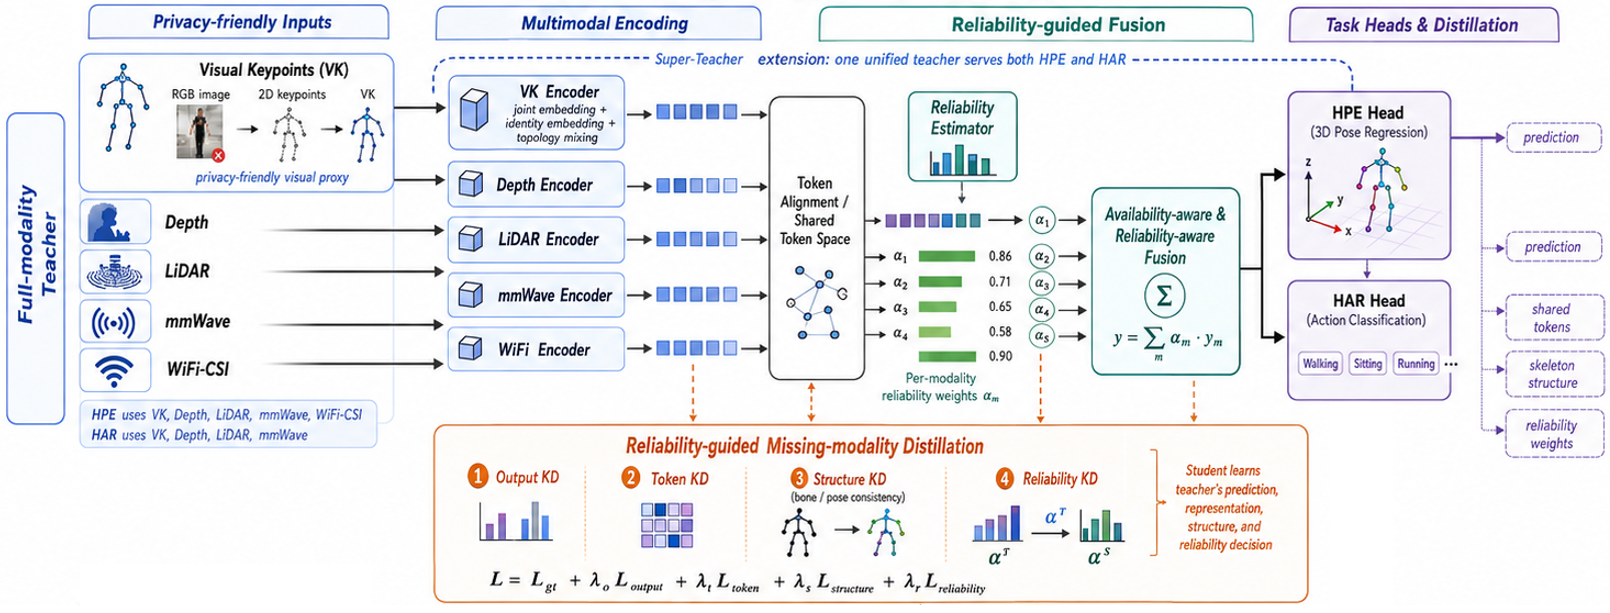
\includegraphics[width=0.98\textwidth]{overall_framework.png}
	\caption{Overall framework of \method{} drawn by the author. Raw RGB is removed and replaced by VK. The full-modality teacher provides privileged supervision, while Student-VK and Student-NV are trained with modality dropping and reliability-aware fusion for incomplete-modality deployment.}
	\label{fig:framework}
\end{figure*}

\section{Experiments}
\subsection{Experimental Setting}
Experiments are conducted on \mmfi{} following the \xfi{}-style protocols. HPE uses VK, depth, LiDAR, mmWave, and WiFi-CSI. HAR uses VK, depth, LiDAR, and mmWave. HPE is evaluated by MPJPE and PA-MPJPE in millimeters; lower values are better. HAR is evaluated by accuracy and macro-F1; higher values are better. The official \xfi{} values are used as public baselines. The notation I/VK means that official \xfi{} uses RGB image input at the corresponding position, whereas this paper uses VK. This is a privacy-oriented replacement rather than an identical input comparison.

Three evaluation protocols are considered when the corresponding results are available. The random split measures in-distribution performance under the same dataset distribution. The cross-scene split evaluates whether a model trained on several environments can transfer to a held-out environment. The cross-subject split evaluates whether the learned representation generalizes to unseen subjects. For missing-modality evaluation, all non-empty modality combinations are tested: 31 combinations for HPE Student-VK, 15 combinations for HAR Student-VK, and 7 combinations for non-visual HAR Student-NV. This design avoids reporting only the easiest full-modality setting.

The comparison with official \xfi{} must be interpreted carefully. Official \xfi{} uses RGB image input for the visual branch, while this paper uses VK. Therefore, I/VK does not mean that the two methods receive identical raw information. The comparison instead asks whether a privacy-oriented structured visual representation can reach or exceed the public \xfi{} baseline under the same task and similar modality positions.

\subsection{HPE Results}
Table~I reports the main HPE results. Student-VK reaches 50.17 mm MPJPE under the full modality setting, improving over the official \xfi{} value of 83.70 mm. Student-NV uses only non-visual modalities and is compared with the official D+L+R+W combination.

The main observation is that privacy-aware visual representation does not necessarily reduce pose accuracy. Teacher, Baseline, and Student-VK all outperform the official full-modality number in the synchronized local evaluation. More importantly, Student-NV reaches 51.03 mm MPJPE without VK, which is substantially lower than the official D+L+R+W value of 97.60 mm. This suggests that non-visual sensors can provide enough geometric information for HPE when the fusion model is trained carefully.

\begin{table}[t]
	\caption{HPE random split main results.}
	\label{tab:hpe-main}
	\centering
	\smalltab
	\begin{tabular}{lccc}
		\toprule
		Model & Modalities & MPJPE & PA-MPJPE\\
		\midrule
		Official \xfi{} & I/VK+D+L+R+W & 83.70 & 47.60\\
		Baseline & I/VK+D+L+R+W & 49.14 & 33.48\\
		Teacher & I/VK+D+L+R+W & 48.45 & 33.06\\
		Student-VK & I/VK+D+L+R+W & 50.17 & 33.48\\
		Student-NV & D+L+R+W & 51.03 & 35.69\\
		Official \xfi{} & D+L+R+W & 97.60 & 47.40\\
		\bottomrule
	\end{tabular}
\end{table}

Cross-scene transfer is harder than random split, as shown in Table~II. Student-VK increases from 50.17 mm to 71.70 mm MPJPE under cross-scene evaluation. This indicates that environment shift remains a major challenge for HPE, even though the model remains usable.

The cross-scene gap is meaningful because HPE depends on precise 3D localization rather than only coarse action semantics. A new environment can change sensor geometry, WiFi propagation, point-cloud density, and background structure. Student-VK has a smaller MPJPE increase than Teacher in Table~II, which is consistent with its missing-modality training objective: the student is repeatedly exposed to incomplete and perturbed sensor evidence, making it less tied to a single ideal full-modality condition.

\begin{table}[t]
	\caption{HPE cross-scene migration.}
	\label{tab:hpe-cross}
	\centering
	\smalltab
	\begin{tabular}{lccc}
		\toprule
		Model & Random MPJPE & Cross MPJPE & Increase\\
		\midrule
		Teacher & 48.45 & 76.06 & +27.61\\
		Student-VK & 50.17 & 71.70 & +21.53\\
		Student-NV & 51.03 & 78.96 & +27.93\\
		\bottomrule
	\end{tabular}
\end{table}

Table~III summarizes 31 Student-VK modality combinations by the number of available modalities. Performance improves as more modalities are available. The average MPJPE over all combinations is 75.18 mm, and the full-modality combination is the best case.

The best single-modality HPE result comes from depth, while LiDAR and WiFi-only settings are weaker. This trend is consistent with the nature of the task: depth directly captures human geometry, whereas wireless and sparse point signals need stronger inference to recover joint-level 3D positions. As the number of modalities increases, the model becomes less dependent on any single weak sensor. The four-modality and five-modality averages are close, showing that much of the benefit can already be obtained before all sensors are available.

\begin{table}[t]
	\caption{HPE Student-VK modality-combination summary.}
	\label{tab:hpe-combo}
	\centering
	\smalltab
	\begin{tabular}{ccccc}
		\toprule
		Available & Comb. & MPJPE & PA-MPJPE & Best MPJPE\\
		\midrule
		1 & 5 & 124.76 & 68.01 & D / 53.88\\
		2 & 10 & 78.10 & 46.85 & I/VK+D / 51.65\\
		3 & 10 & 60.78 & 38.08 & I/VK+D+R / 50.50\\
		4 & 5 & 53.55 & 34.89 & I/VK+D+L+R / 50.25\\
		5 & 1 & 50.17 & 33.48 & All / 50.17\\
		\bottomrule
	\end{tabular}
\end{table}

\subsection{HAR Results}
Table~IV reports HAR results. Student-VK improves the full-modality random accuracy from the official \xfi{} value of 72.20\% to 96.56\%. Under cross-scene and cross-subject settings, the full-combination accuracies remain above 95\%. Student-NV also performs strongly, indicating that non-visual deployment is feasible for HAR.

HAR behaves differently from HPE. Action labels are more tolerant to small spatial errors, and temporal or geometric patterns can be sufficient to distinguish many actions. This explains why Student-NV remains above 95\% in all three full-combination protocols. The result is practically important: for many indoor monitoring applications, recognizing the activity may be more important than reconstructing an accurate 3D skeleton, and this can be achieved without raw RGB or even VK.

\begin{table}[t]
	\caption{HAR main results.}
	\label{tab:har-main}
	\centering
	\smalltab
	\begin{tabular}{llcc}
		\toprule
		Protocol & Model & Acc. & Macro-F1\\
		\midrule
		Random & Teacher & 95.57 & 95.56\\
		Random & Student-VK & 96.56 & 96.55\\
		Random & Student-NV & 96.12 & 96.13\\
		Cross-scene & Teacher & 94.80 & 94.83\\
		Cross-scene & Student-VK & 95.25 & 95.25\\
		Cross-scene & Student-NV & 95.41 & 95.40\\
		Cross-subject & Teacher & 95.52 & 95.48\\
		Cross-subject & Student-VK & 96.12 & 96.10\\
		Cross-subject & Student-NV & 95.70 & 95.67\\
		\bottomrule
	\end{tabular}
\end{table}

Table~V reports average HAR accuracy over all modality combinations. Student-VK achieves 85.15\%, 80.61\%, and 85.30\% average accuracy on random, cross-scene, and cross-subject protocols, respectively. Student-NV is lower on average but remains practical without visual input.

The average-combination results are lower than full-combination results because they include difficult single-modality cases. This is expected and should not be hidden. A robust deployment model should degrade gracefully when sensors are missing. In the random protocol, Student-VK averages 85.15\% over all 15 combinations, while Student-NV averages 80.62\% over its 7 non-visual combinations. Cross-scene is the hardest protocol for HAR combination robustness, especially for weak single-modality settings, but full-combination Student-NV still remains competitive.

\begin{table}[t]
	\caption{HAR modality-combination robustness.}
	\label{tab:har-combo}
	\centering
	\smalltab
	\begin{tabular}{llccc}
		\toprule
		Protocol & Model & Comb. & Avg. Acc. & Avg. F1\\
		\midrule
		Random & Student-VK & 15 & 85.15 & 85.15\\
		Cross-scene & Student-VK & 15 & 80.61 & 80.35\\
		Cross-subject & Student-VK & 15 & 85.30 & 85.46\\
		Random & Student-NV & 7 & 80.62 & 80.48\\
		Cross-scene & Student-NV & 7 & 76.70 & 76.41\\
		Cross-subject & Student-NV & 7 & 81.26 & 80.82\\
		\bottomrule
	\end{tabular}
\end{table}

\subsection{Ablation and Robustness}
Table~VI compares distillation and fusion variants. On HAR, removing distillation or using uniform fusion reduces accuracy. On HPE, some distillation variants achieve slightly lower MPJPE than the default Student-VK, suggesting that the loss balance should be further tuned. However, uniform fusion is clearly worse for HPE, supporting the need for reliability-aware fusion.

The ablation results show that the contribution of each module is task-dependent. For HAR, the complete Student-VK is stronger than NoKD and Uniform, which supports the distillation and reliability-aware design. For HPE, Output KD and NoKD produce competitive MPJPE in the current single-run results, but Uniform fusion still degrades both MPJPE and PA-MPJPE. A conservative interpretation is therefore that reliability-aware fusion is consistently useful, while the best distillation loss balance for HPE requires further repeated experiments.

\begin{table}[t]
	\caption{Ablation study.}
	\label{tab:ablation}
	\centering
	\smalltab
	\begin{tabular}{lccc}
		\toprule
		Setting & HPE MPJPE & HPE PA & HAR Acc.\\
		\midrule
		Student-VK & 50.17 & 33.48 & 96.54\\
		NoKD & 48.83 & 32.51 & 95.97\\
		Output KD & 47.62 & 32.15 & --\\
		Output+Token KD & 48.76 & 33.24 & --\\
		Output+Bone KD & 49.34 & 33.38 & --\\
		Uniform fusion & 52.28 & 37.22 & 95.40\\
		\bottomrule
	\end{tabular}
\end{table}

VK robustness is evaluated by adding coordinate noise and randomly dropping joints. Without perturbation, Student-VK obtains 50.18 mm MPJPE. With 50\% joint dropping and no coordinate noise, MPJPE increases to 54.75 mm. With noise standard deviation 20 and 50\% joint dropping, MPJPE is 54.78 mm. This small degradation shows that the multimodal model does not rely on a perfectly clean VK signal.

\begin{table}[t]
	\caption{VK perturbation robustness on HPE Student-VK.}
	\label{tab:vk-robust}
	\centering
	\smalltab
	\begin{tabular}{cccc}
		\toprule
		Noise std. & Joint drop & MPJPE & PA-MPJPE\\
		\midrule
		0 & 0\% & 50.18 & 33.47\\
		0 & 50\% & 54.75 & 36.03\\
		20 & 0\% & 50.20 & 33.47\\
		20 & 50\% & 54.78 & 36.04\\
		\bottomrule
	\end{tabular}
\end{table}

\begin{table}[t]
	\caption{HPE model complexity in synchronized results.}
	\label{tab:complexity}
	\centering
	\smalltab
	\begin{tabular}{lccc}
		\toprule
		Model & Params & FPS & Peak Memory\\
		\midrule
		Baseline & 5.74M & 52.04 & 4.60 GB\\
		Teacher & 8.90M & 63.24 & 4.61 GB\\
		Student-VK & 8.90M & 62.01 & 4.61 GB\\
		Student-NV & 8.90M & 63.37 & 4.61 GB\\
		\bottomrule
	\end{tabular}
\end{table}

Table~VIII gives the synchronized HPE complexity values. The students keep a similar parameter count and memory footprint to the teacher because they reuse the same projected multimodal architecture while changing the available modality set. The important deployment gain is therefore not only parameter reduction, but input flexibility: the same trained student can be evaluated under many modality subsets without training a separate model for each subset.

\subsection{Deployment-Oriented Synthesis}
The experiments can be summarized by deployment mode rather than by model name alone. Table~IX presents this view. When all sensors are available and privacy constraints are moderate, Student-VK is the most balanced choice because it keeps VK and non-visual modalities. When cameras are not acceptable, Student-NV provides a direct non-visual solution. When a system is used in a new room, cross-scene results should be prioritized over random-split results. When sensors may fail dynamically, average performance over all modality combinations is more informative than the full-combination score.

\begin{table}[t]
	\caption{Scenario-oriented interpretation of the current results.}
	\label{tab:deployment}
	\centering
	\smalltab
	\begin{tabular}{lcc}
		\toprule
		Scenario & Recommended model & Main evidence\\
		\midrule
		Full sensors & Student-VK & HPE 50.17 mm, HAR 96.56\%\\
		No visual input & Student-NV & HPE 51.03 mm, HAR 96.12\%\\
		New environment & Student-VK/NV & Cross-scene HAR $>$95\%\\
		Sensor missing & Student-VK & 31/15 combination tests\\
		Privacy sensitive & Student-NV & No RGB and no VK\\
		\bottomrule
	\end{tabular}
\end{table}

This synthesis is also useful for explaining why the teacher is not the main deployment result. A full-modality teacher can be strong, but it assumes that every sensor is available and clean. In a real deployment, this assumption is fragile. The student models intentionally sacrifice a small amount of ideal full-modality performance to gain broad compatibility with incomplete inputs. In the current experiments, the sacrifice is small: Student-VK is close to the teacher in both HPE and HAR, while being trained for arbitrary modality subsets.

The most difficult cases reveal where future improvements should focus. In HPE, single LiDAR or single WiFi combinations remain weak because they do not directly provide dense body geometry. In HAR, some single-modality LiDAR combinations are unstable, especially under cross-scene evaluation. These cases suggest that the next algorithmic step should not simply add a larger backbone. A more targeted direction is to estimate sensor confidence explicitly, use corruption-aware training, and let the fusion module learn when to suppress sparse or unreliable tokens.

\section{Discussion and Limitations}
The results support three findings. First, replacing raw RGB with VK can preserve strong performance while reducing direct exposure of identity and background information. Second, missing-modality training is necessary because the full-modality teacher is not a deployment model for arbitrary incomplete inputs. Third, non-visual deployment is feasible, especially for HAR, where Student-NV reaches 96.12\% random accuracy.

Table~X summarizes the deployment meaning of different input choices. Raw RGB provides the richest visual information but exposes face, clothing, and background cues. VK removes image texture and keeps only joint coordinates, which is more suitable for privacy-sensitive monitoring. Depth, LiDAR, mmWave, and WiFi-CSI further reduce visual exposure, but each non-visual modality has its own weakness. For example, LiDAR and mmWave may become sparse, and WiFi-CSI is sensitive to environment changes. Therefore, the practical value of \method{} is not only higher accuracy, but also the ability to select a deployment point between privacy, robustness, and sensor availability.

\begin{table}[t]
	\caption{Qualitative privacy and deployment comparison.}
	\label{tab:privacy}
	\centering
	\smalltab
	\begin{tabular}{lccc}
		\toprule
		Input & Texture & Background & Deployment role\\
		\midrule
		RGB & High & High & Strong but privacy-sensitive\\
		VK & Low & Low & Structured visual substitute\\
		Depth/LiDAR & Low & Medium & Geometry-aware sensing\\
		mmWave/WiFi & Very low & Low & Non-visual sensing\\
		\bottomrule
	\end{tabular}
\end{table}

The current experiments also indicate that the method should be evaluated by deployment scenarios instead of by a single full-modality score. If all sensors are available, the full-modality teacher and Student-VK provide strong HPE and HAR performance. If visual information is restricted, Student-NV provides a direct non-visual alternative. If sensors are partially unavailable, the randomly dropped Student-VK is more appropriate than a full-modality-only model. This scenario-based interpretation is important because real systems rarely operate under a fixed and perfect sensor configuration.

Another observation is that HPE and HAR should not be judged by the same failure pattern. HPE is more sensitive to calibration, coordinate accuracy, and environment geometry. HAR is more robust because many actions can be recognized from coarser temporal patterns. This explains why cross-scene degradation is more visible in HPE than in HAR. It also suggests a practical deployment strategy: when a system requires precise rehabilitation measurement or robotic interaction, cross-scene calibration should be prioritized; when the system only requires action-level monitoring, a non-visual HAR model may already be sufficient.

There are also limitations. The comparison between official RGB and VK is not a strictly identical input comparison. VK is a structured representation and should be interpreted as a privacy-oriented deployment alternative rather than a direct RGB backbone replacement. HPE cross-subject experiments are not yet fully synchronized locally, so they are not used as a main conclusion. In addition, current reported values are mainly from single completed runs. Repeated experiments with multiple random seeds would provide stronger statistical evidence.

The privacy claim is also qualitative in the current version. Removing raw RGB clearly reduces direct visual exposure, but a stronger study should quantify privacy leakage. Possible tests include identity recognition from RGB versus VK, background classification from visual inputs, and reconstruction risk from stored representations. Such analysis would make the privacy-preserving claim more rigorous. Similarly, the current method sanitizes sparse or empty mmWave frames during data loading, but future work should explicitly report sensor failure statistics and evaluate whether reliability weights correlate with sensor quality.

For a course project, the most important technical lesson is that robustness should be designed jointly at the data, model, and evaluation levels. Random modality dropping creates incomplete inputs during training. Distillation prevents the student from learning only from sparse ground-truth supervision. Reliability-aware fusion provides a lightweight mechanism to reduce the effect of weak modality subsets at inference time. The experiments therefore evaluate not only whether one model is accurate, but also whether the same training pipeline can support several realistic deployment modes: full-sensor, partial-sensor, and non-visual sensing.

Overall, the current work is best understood as a robust deployment-oriented extension of \xfi{} rather than as a new dataset or a completely new sensing backbone. Its value comes from combining a privacy-preserving input policy, arbitrary missing-modality training, non-visual evaluation, and reliability-aware decision fusion into one consistent experimental pipeline. The remaining research gap is to sharpen the algorithmic novelty further, for example by making reliability estimation explicitly uncertainty-calibrated or by learning modality-specific confidence targets from sensor corruption statistics.

\section{Conclusion}
This paper presented \method{}, a privacy-preserving and missing-modality robust multimodal human sensing framework. By replacing raw RGB with VK, distilling full-modality knowledge to missing-modality students, and using reliability-aware fusion, \method{} supports HPE and HAR under diverse modality subsets. The current results show strong full-modality performance, practical non-visual deployment, and meaningful robustness to missing or noisy inputs. The complete story is therefore not only that VK can replace RGB in a model branch, but that multimodal human sensing can be redesigned around privacy constraints and sensor availability. Future work should complete HPE cross-subject evaluation, run multi-seed significance tests, and provide a more quantitative privacy leakage analysis.

% ---------------- References ----------------
\begin{thebibliography}{99}
	\bibitem{xfi} X. Chen and J. Yang, ``X-Fi: A modality-invariant foundation model for multimodal human sensing,'' in \textit{Proc. Int. Conf. Learn. Represent.}, 2025.
	\bibitem{mmfi} J. Yang, H. Huang, Y. Zhou, X. Chen, Y. Xu, S. Yuan, H. Zou, C. X. Lu, and L. Xie, ``MM-Fi: Multi-modal non-intrusive 4D human dataset for versatile wireless sensing,'' in \textit{Proc. Adv. Neural Inf. Process. Syst. Datasets and Benchmarks Track}, 2023.
	\bibitem{hinton} G. Hinton, O. Vinyals, and J. Dean, ``Distilling the knowledge in a neural network,'' \textit{arXiv preprint arXiv:1503.02531}, 2015.
	\bibitem{incompletekd} Q. Wang, C. Zhan, P. Thompson, and J. Zhou, ``Multimodal learning with incomplete modalities by knowledge distillation,'' in \textit{Proc. ACM SIGKDD Int. Conf. Knowl. Discov. Data Mining}, 2020.
	\bibitem{lckd} C. Pham, P. P. Liang, T. Manzini, L. Morency, and B. Poczos, ``Found in translation: Learning robust joint representations by cyclic translations between modalities,'' in \textit{Proc. AAAI Conf. Artif. Intell.}, 2019.
	\bibitem{smil} M. Ma, J. Ren, L. Zhao, S. Tulyakov, C. Wu, and X. Peng, ``SMIL: Multimodal learning with severely missing modality,'' in \textit{Proc. AAAI Conf. Artif. Intell.}, 2021.
	\bibitem{missingtransformer} M. Ma, J. Ren, L. Zhao, D. Testuggine, and X. Peng, ``Are multimodal transformers robust to missing modality?'' in \textit{Proc. IEEE/CVF Conf. Comput. Vis. Pattern Recognit.}, 2022.
	\bibitem{paramadapt} M. K. Reza, A. Prater-Bennette, and M. S. Asif, ``Robust multimodal learning with missing modalities via parameter-efficient adaptation,'' \textit{IEEE Trans. Pattern Anal. Mach. Intell.}, 2025.
	\bibitem{dynamicfusion} Z. Xue and R. Marculescu, ``Dynamic multimodal fusion,'' in \textit{Proc. IEEE/CVF Conf. Comput. Vis. Pattern Recognit.}, 2023.
	\bibitem{stgcn} S. Yan, Y. Xiong, and D. Lin, ``Spatial temporal graph convolutional networks for skeleton-based action recognition,'' in \textit{Proc. AAAI Conf. Artif. Intell.}, 2018.
	\bibitem{pointtransformer} H. Zhao, L. Jiang, J. Jia, P. H. S. Torr, and V. Koltun, ``Point transformer,'' in \textit{Proc. IEEE/CVF Int. Conf. Comput. Vis.}, 2021, pp. 16259--16268.
	\bibitem{transformer} A. Vaswani, N. Shazeer, N. Parmar, J. Uszkoreit, L. Jones, A. N. Gomez, L. Kaiser, and I. Polosukhin, ``Attention is all you need,'' in \textit{Proc. Adv. Neural Inf. Process. Syst.}, 2017.
	\bibitem{widar} Y. Zheng, Y. Zhang, K. Qian, G. Zhang, Y. Liu, C. Wu, and Z. Yang, ``Zero-effort cross-domain gesture recognition with Wi-Fi,'' in \textit{Proc. ACM MobiSys}, 2019.
	\bibitem{radhar} S. Singh, S. A. Velastin, and H. Ragheb, ``RadHAR: Human activity recognition from point clouds generated through a millimeter-wave radar,'' in \textit{Proc. ACM Workshop on Millimeter-Wave Networks and Sensing Systems}, 2019.
	\bibitem{privacysurvey} A. S. R. S. A. K. Jalal, S. Kamal, and D. Kim, ``A depth video sensor-based life-logging human activity recognition system for elderly care in smart indoor environments,'' \textit{Sensors}, vol. 14, no. 7, pp. 11735--11759, 2014.
\end{thebibliography}

% Blank page for the course requirement: the submitted PDF should have an even number of pages
% and stay within the required 5--8 page range under the IEEEtran two-column template.
\clearpage
\mbox{}
\thispagestyle{empty}
\clearpage

\end{document}
